\documentclass[a4paper,11pt]{jlreq}
% 基本とドライバ関連
\usepackage{graphicx}
\usepackage{xcolor}
\usepackage{makeidx}
\usepackage{ascmac}

% LuaTeX-ja設定
\usepackage{luatexja}% 日本語したい
\usepackage[haranoaji,no-math,deluxe,expert,nfssonly,match,scale=1.0]{luatexja-preset}
\renewcommand{\kanjifamilydefault}{\gtdefault}% 既定をゴシック体に
\usepackage{lltjext}

% 数式系基本
\usepackage{amsmath}
\usepackage{amsthm}
\usepackage{amssymb}
\usepackage{mathtools}
% \mathtoolsset{showonlyrefs=true}
\usepackage{derivative}
\usepackage[b]{esvect}
\usepackage{nicematrix}
\usepackage{siunitx}
\usepackage{bm}

% 画像関係
\usepackage{animate}
\usepackage{svg}
\usepackage{tikz}

%表関連
\usepackage{multirow}

% 自然科学用追加
% \usepackage{chemmacros}
% \usechemmodule{all}
% \selectchemgreekmapping{fontspec}
\usepackage{chemfig}
\setchemfig{atom sep=1.5em}
% \ifdraft{}{\setchemfig{bond join=true}}

% 数式フォント設定
\usepackage{anyfontsize}
\newcommand{\sfscale}{0.98}
\newcommand{\ttscale}{0.96}
% \usepackage[mathnoalias]{iwona}
% % \setmainfont{Iwona}
% \usepackage[scale=\sfscale]{roboto}
% \usepackage[scale=\ttscale]{roboto-mono}
% \usepackage{BOONDOX-uprscr}
% \usepackage{BOONDOX-ds}

% ページ設定
\usepackage{geometry}
\geometry{left=25truemm, right=25truemm, top=25truemm, bottom=25truemm}
% \pagestyle{empty}

% hyperref関連
\usepackage{bookmark}
\usepackage{xurl}
\hypersetup{unicode,bookmarksnumbered=true,colorlinks=true,final}

%%%%%%%%%%%%%%%%%%%%%%%
\graphicspath{{../figure/}{../../figure/}}

\begin{document}
\section{炭素の結合角}
\label{sec: carbon_BA}

炭素の結合角が、約\qty{109.5}{\degree}であることを確認しよう。

炭素のそれぞれの結合を図示すると、下図に示したように正四面体の重心に着目する炭素が、また、各頂点にそれぞれの原子が配置されることになる。

\begin{center}
	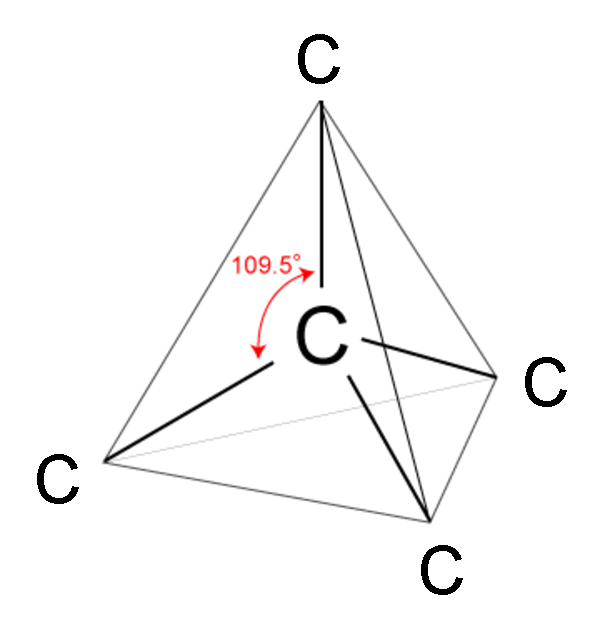
\includegraphics[width=.3\textwidth]{carbon.eps}
\end{center}

\subsection{幾何学的なやり方}

この正四面体の各頂点を A, B, C, D とし、各辺の長さを1とする。
また、重心を G、辺 BC の中点を M とし、さらに、頂点 A から $\bigtriangleup$ BCD に下した垂線の足を K とする。


\begin{center}
	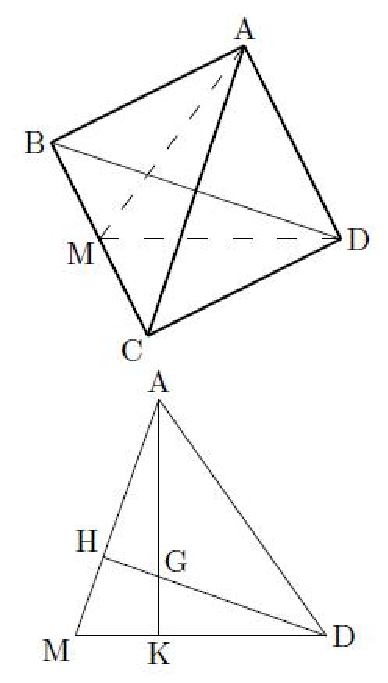
\includegraphics[width=.3\textwidth]{Carbon_BA.pdf}
\end{center}
この設定の元で、結合角(例えば、$\angle$ AGD)を求めよう。

まず、$\bigtriangleup$ CDM において、$\angle$ DMC = $\perp$, $\angle$ DCM =\qty{60}{\degree}であるので、
\begin{align*}
{\mathrm CM} : {\mathrm CD} : {\mathrm DM} &= 1: 2 : \sqrt{3} \\
\therefore \quad {\mathrm DM} &= \dfrac{\sqrt{3}}{2}
\end{align*}

次に、$\bigtriangleup$ KBC に着目すると、$\angle$ BKC =\qty{120}{\degree}より $\angle$ BKM = \qty{60}{\degree} であるので MK:KB=1:2 となる。
また、Kは$\bigtriangleup$BCDの重心であるのでKB=KD、したがって、
\begin{align*}
{\mathrm DM} &= {\mathrm MK} + {\mathrm KD} = {\mathrm MK} + {\mathrm KB} = 3 \times {\mathrm MK} \\
\therefore \quad {\mathrm MK} 
	&=\dfrac{ {\mathrm DM} }{3} \\
	&=\dfrac{\sqrt{3}}{6}
\end{align*}

AM=DM であることに注意すると、$\bigtriangleup$ AMK において三平方の定理より、
\begin{align*}
{\mathrm AK} 
	&= \sqrt{ {\mathrm AM}^2 - {\mathrm MK}^2 } \\
	&= \dfrac{\sqrt{6}}{3}
\end{align*}

$\bigtriangleup$ AMK $\sim$ $\bigtriangleup$ AGH であるので、AM:AG = AK:AH となり、
\begin{align*}
{\mathrm AG} 
	&= { {\mathrm AM} } \times \dfrac{ {\mathrm AK} }{ {\mathrm AH} } \\
	&= { {\mathrm AM} } \times \dfrac{ {\mathrm AK} }{ ({\mathrm AM} - {\mathrm HM}) } \\
	&= \dfrac{\sqrt{3}}{2} \times \dfrac{ \dfrac{\sqrt{6}}{3} }{ \left( \dfrac{\sqrt{3}}{2} - \dfrac{\sqrt{3}}{6} \right) } \\
%	&= \dfrac{\sqrt{3}}{2} \times \dfrac{ \dfrac{\sqrt{6}}{3} }{ \dfrac{2\sqrt{3}}{3} } \\
	&= \dfrac{ \sqrt{6} }{ 4 }
\end{align*}

この時、求める結合角 $\angle$ AGD は、$\bigtriangleup$ AGD に対して余弦定理
\footnote{
    三角形の辺の長さと内角の余弦の間に成り立つ関係を与える定理であり、
    $\bigtriangleup$ ABC において、a = BC, b = CA, c = AB, $\alpha$ = $\angle$ CAB, $\beta$ = $\angle$ ABC, $\gamma$ = $\angle$ BCA としたとき
    \begin{align*}
    a^2 &= b^2 + c^2 − 2 bc \cos \alpha \\
    b^2 &= c^2 + a^2 − 2 ca \cos \beta \\
    c^2 &= a^2 + b^2 − 2 ab \cos \gamma
    \end{align*}
    と表される。
    }
を用いて、
\begin{align*}
\cos \angle {\mathrm AGD} 
	&= \dfrac{ {\mathrm AG}^2 + {\mathrm GD}^2 - {\mathrm AD}^2 }{ 2 \times {\mathrm GA} \times {\mathrm GD} } \\
	&= \dfrac{ \left( \dfrac{ \sqrt{6} }{ 4 } \right)^2 + \left( \dfrac{ \sqrt{6} }{ 4 } \right)^2 - \left( 1 \right)^2 }{ 2 \times \dfrac{ \sqrt{6} }{ 4 } \times \dfrac{ \sqrt{6} }{ 4 } } \\
%	&= \dfrac{ \dfrac{ 12 }{ 16 } -1 }{\dfrac{ 12 }{ 16 }} \\
	&= -\dfrac{ 1 }{ 3 }
\end{align*}
となる。

関数電卓等を用いて、
\begin{align*}
\angle {\mathrm AGD} = \cos ^{-1} \left( -\dfrac{1}{3} \right) = 109.4712206 \cdots
\end{align*}
という無理数の形で得られるので、これを小数第一位で丸めて、約 \qty{109.5}{\degree} と表記しているわけです。

\subsection{ベクトル形式での解法}

重心 G から各頂点( A, B, C, D )への長さが 1 の正四面体を考えよう。
これをベクトルで、$\overrightarrow{GA} = {\bm a}, \overrightarrow{GB} = {\bm b}, \cdots$ と表し、
結合角(例えば、$\angle AGB$ )を $\theta$ と表記しよう。

このとき、
\begin{align*}
&{\bm a} \cdot {\bm b} = {\bm a} \cdot {\bm c} = {\bm a} \cdot {\bm d} = {\bm b} \cdot {\bm c} = {\bm b} \cdot {\bm d} = {\bm c} \cdot {\bm d} = 1 \times 1 \times \cos \theta = \cos \theta \\
&|{\bm a}|^2 = |{\bm b}|^2 = |{\bm c}|^2 = |{\bm d}|^2 = 1
\end{align*}
となる。

また、重心の定義より、
\begin{align*}
{\bm a} + {\bm b} + {\bm c} + {\bm d} = {\bm 0} \\
\therefore \quad -{\bm d} ={\bm a} + {\bm b} + {\bm c}
\end{align*}

したがって、
\begin{align*}
|{\bm d} | 
	&= |{\bm a} + {\bm b} + {\bm c}| \\
	&= \sqrt{ |{\bm a}|^2 + |{\bm b}|^2 + |{\bm c}|^2 + 2{\bm a}{\bm b} + 2{\bm a}{\bm c} + 2{\bm b}{\bm c} } \\
	&= \sqrt{ 3 + 6 \cos \theta } \\
	&= 1 \\
\therefore \quad \cos \theta &= -\dfrac{1}{3}
\end{align*}
を得る。

\end{document}